\documentclass[12pt]{report}
\usepackage[utf8]{inputenc}
\usepackage[french]{babel}
\usepackage[T1]{fontenc}
\usepackage{xcolor}
\usepackage{listings}
\usepackage{graphicx}
\renewcommand{\thechapter}{}
%\renewcommand{\thesection}{}
\renewcommand*\thesection{\arabic{section}}
\setcounter{chapter}{1}
\addto\captionsfrench{
  \renewcommand\chaptername{}}
\title{Rapport de projet NachOS}
\author{
\'Equipe H\\\\
Mohd Thaqif ABDULLAH HASIM\\
Florian BARROIS\\
Cédric GARCIA\\
Hosseim NAHAL\\
Peio RIGAUX\\
}

\begin{document}
\maketitle


\chapter{Présentation de \color{red}notre nom badass\color{black}}

est un système d'exploitation basé sur le fonctionnement du système Unix. Il propose ainsi une version simplifiée des fonctionnalités de ce dernier, à savoir :
\begin{itemize}%[label=\textbullet,font=\color{black}]
\item Un système synchronisé d'entrées/sorties;
\item La gestion de plusieurs processus utilisateurs multithreadés \color{red}SI ON ARRIVE A FAIRE FONCTIONNER LES TESTS !\color{black}
\item Un système de fichiers permettant la manipulation de fichiers et la navigation à travers les répertoires \color{red}GERANT LES FICHIERS OUVERTS ??\color{black} et dont la taille des fichiers peut atteindre 112,5Ko.
\item La possibilité de communiquer en réseau...\color{red}DETAILS\color{black}

\end{itemize}


\chapter{Spécifications}
\section{Entrées/Sorties}

\textbf{char GetChar():}

Retourne le caractère lu sur l'entrée standard.\\


\textbf{void PutChar(char c):}

Écrit le caractère c sur la sortie standard.\\


\textbf{void GetString(char* s, int n)}
\color{red} FONCTION DE LA MORT ! GROS BORDEL
Récupère n caractères depuis l'entrée standard et les stocke dans la  variable s. Si le caractère de saut de ligne '\textbackslash n' se trouve dans la chaîne à lire, alors seuls les caractères lus jusqu'ici, '\textbackslash n' exclus, sont stockés dans s. Les caractères restants sont stockés dans \color{black}




 n premiers caractères est le caractère de saut de ligne '\textbackslash n', alors la lecture s'arrête et s contient tous les le reste de la chaîne est ignorélecture s’arrête lorsqu’un ‘\textbackslash n’ ou EOF est rencontré.
‘\textbackslash 0’ est stocké après le dernier caractère dans le tampon s.
‘\textbackslash 0’ est stocké à l’indice 0 du tampon quand la fin du fichier est détectée alors qu’aucun caractère n’a été lu.

\textbf{void PutString(const char s*)}

Parcourt la chaîne de caractères s et écrit caractère par caractère sur la sortie définie précédemment jusqu’à la rencontre du caractère ‘\textbackslash 0’ ou jusqu’à ce que MAX\_STRING\_SIZE soit atteinte. Le comportement est indéfini dans le cas où s ne contient pas de ‘\textbackslash 0’.

\textbf{void GetInt(int* n)}

Lit un entier depuis l'entrée standard, si la valeur n'est pas dans [$-2^{31}$; $2^{31}-1$] elle sera forcée à une de ces valeurs (la limite est de 16 caractères pour les entiers, au-delà les caractères ne seront pas comptés). SI un utilisateur entre le signe ‘-’ sans le faire suivre de chiffres, la valeur 0 est stockée.

\textbf{void PutInt(int n)}

Récupère la valeur de l’entrée définie précédemment puis l’écrit à l’adresse pointée par n. Le comportement est indéfini si la valeur n'est pas dans [$-2^{31}$; $2^{31}-1$].

\bigskip

\section{Threads, processus et synchronisation}
\bigskip

\textbf{int UserThreadCreate(int f, int arg):}

Initialise un thread utilisateur qui appelle la fonction f avec l'argument arg. Bien que UserThreadCreate autorise un seul argument pour la fonction f, il est possible de lui transmettre plusieurs arguments en les définissant comme paramètres d'une structure.
Retourne l’identifiant du thread créé.
\bigskip

\textbf{void UserThreadJoin(int tid):}

Interrompt l'exécution du thread appelant jusqu'à la terminaison du thread identifié par tid.
\bigskip


\textbf{void UserThreadExit():}

Termine l'exécution du thread appelant. L'appel à UserThreadExit() est facultatif puisqu'il est systématiquement réalisé lorsqu'un thread a terminé l'exécution de la fonction qui lui a été attribuée. Il peut néanmoins être utilisé pour forcer l'arrêt du thread avant la fin de sa tâche.
\bigskip


\textbf{void Sem\_init(Semaphore* sem, int val):}

Initialise la valeur du sémaphore sem à val.
\bigskip	


\textbf{void Sem\_wait(Semaphore sem):}

Décrémente la valeur du sémaphore sem. Sem\_wait est bloquant tant que la valeur de sem est égale à zéro, empêchant ainsi la décrémentation.
L'appel à Sem\_wait nécessite que le sémaphore sem ait été initialisé avec la fonction Sem\_init.
\bigskip


\textbf{void Sem\_post(Semaphore sem):}

Incrémente la valeur du sémaphore sem. Si, une fois incrémentée, la valeur de sem vaut un alors qu'un fil d'exécution est bloqué par Sem\_wait sur le même sémaphore sem, alors ce fil d'exécution reprend son activité.
L'appel à Sem\_post nécessite que le sémaphore sem ait été initialisé avec la fonction Sem\_init.
\bigskip


\textbf{void Sem\_destroy(Semaphore sem):}

Détruit le sémaphore sem. Si sem est détruit alors que des fils d'exécution ont été suspendus par un appel à Sem\_wait sur ce même sémaphore sem, ces fils d'exécution ne se termineront pas avant l'arrêt complet du système.\\
\color{red}Potentiellement à tester mais devrait être le comportement logique\color{black}
\bigskip


\textbf{void ForkExec(char* filename):}

Crée un nouveau processus qui exécute le programme passé en paramètre. \'A sa création, le nouveau processus contient un seul fil d'exécution. Les valeurs des registres de ce fil d'exécution sont identiques à celles des registres du fil d'exécution qui a appelé ForkExec.
\bigskip


\section{Système de fichiers}


\section{Réseau}
\color{red}PAS DE RESEAU PUISQUE PAS DU COTE USER ?\color{black}


\chapter{Tests utilisateur}
\section{Test sur la console :}
Pour l’instant, les tests fonctionnent à l’aide de l’entrée/sortie standard et les types de données pouvant être entrés sont testés manuellement (tentative de dépasser la taille que peut stocker un int pour getint.c par exemple).

%putchar.c : Programme donné dans le sujet de l’étape 2 permettant de tester l’appel système PutChar et d’afficher une série de caractères.
%putstring.c : Affiche la chaîne de caractères passé en paramètre de PutString sur la sortie. En cas de chaîne ayant une taille plus grande que MAX\_STRING\_SIZE, PutString n’envoie que les  MAX\_STRING\_SIZE premiers caractères.
getchar.c : Récupère un caractère sur l’entrée puis l’affiche, lui et les deux caractères le suivant dans l’ordre alphabétique.
getstring.c : Demande le nom de l’utilisateur (une chaîne de caractères) puis l’affiche précédé de « Bonjour Monsieur ».
 getint.c : Demande un entier à l’utilisateur, le borne afin de le faire rentrer dans un int, puis l’affiche (Ce test sert à la fois pour SynchGetInt() que pour SynchPutInt()).

\chapter{Implémentation}

\section{Entrées/Sorties}

%char SynchGetChar() :
%Fait appel à la fonction GetChar() de Console pour récupérer un caractère depuis l'entrée standard grâce un mécanisme d'interruption.
%
%void SynchPutChar(const char ch) : 
%Fait appel à la fonction PutChar() de Console pour écrire un caractère ch sur la sortie standard déclenchant une interruption.
%
%void SynchGetString() : 
%Effectue des appels à la fonction SynchGetChar() dans une boucle bornée par le nombre de caractères lus. Le caractère de fin de chaîne est concaténé à la chaîne obtenue.
%
%void SynchPutString(const char s[]) : 
%Fait appel à la fonction SynchPutChar() dans une boucle pour afficher des caractères sur la sortie standard. La boucle s'arrête lorsque le caractère de fin de chaîne est détecté ou lorsque la nombre maximum de caractères est atteint.  
%
%void SynchGetInt(int *n) : 
%Lit une chaîne de caractères depuis l'entrée standard grâce à la fonction SynchGetChar(). Le premier caractère est testé pour pouvoir considérer les nombres négatifs. Ensuite tant qu'un caractère dont le code ASCII correspond à un chiffre est détecté, ce chiffre est ajouté à la chaîne. La chaîne est terminée par le caractère de fin de chaîne et est stockée dans l’entier pointé par n.
%
%void SynchPutInt(const int n) : 
%Convertit l'entier n au format chaîne de caractères et l'affiche sur la sortie standard en appelant la fonction SynchPutString().


\section{Threads}



%int UserThreadCreate(int f, int arg, int fin)
%Initialise un thread utilisateur, l’ajoute à la liste de threads et exécute la fonction f. Au niveau des arguments, f pointe vers la fonction que devra exécuter le thread et arg correspond au paramètre passé à la fonction f. Renvoie l’identifiant du thread.
%
%
%int do\_UserThreadExit()
%Enlève le thread courant de la liste des thread et termine son exécution.
%static void StartUserThread(int f)
%Initialise les registres MIPS et exécute la fonction f.
%static int getIndexThreadById(int id)
%Récupère l’index du thread ayant l’identifiant id dans la liste de threads.

\section{Processus}



\section{Pagination}


Stratégies d’allocation des pages physiques géré par un tirage aléatoire via la méthode « GetEmptyFrame » . Utilisation d’une bitmap pour vérifier si la frame est déjà allouer ou non.\color{red}WHAT ?\color{black}

La fins des processus et des threads est gérée automatiquement via un compteur pour déterminer s'il est nécessaire d'effectuer une interruption machine ou une terminaison de thread.

\section{Système de fichiers}


\section{Réseau}

La partie réseau du système fonctionne grâce à un protocole de communication qui a été créé en se basant sur le fonctionnement du protocole TCP/IP. L'échange d'information s'effectue comme indiqué ci-dessous.

\begin{center}
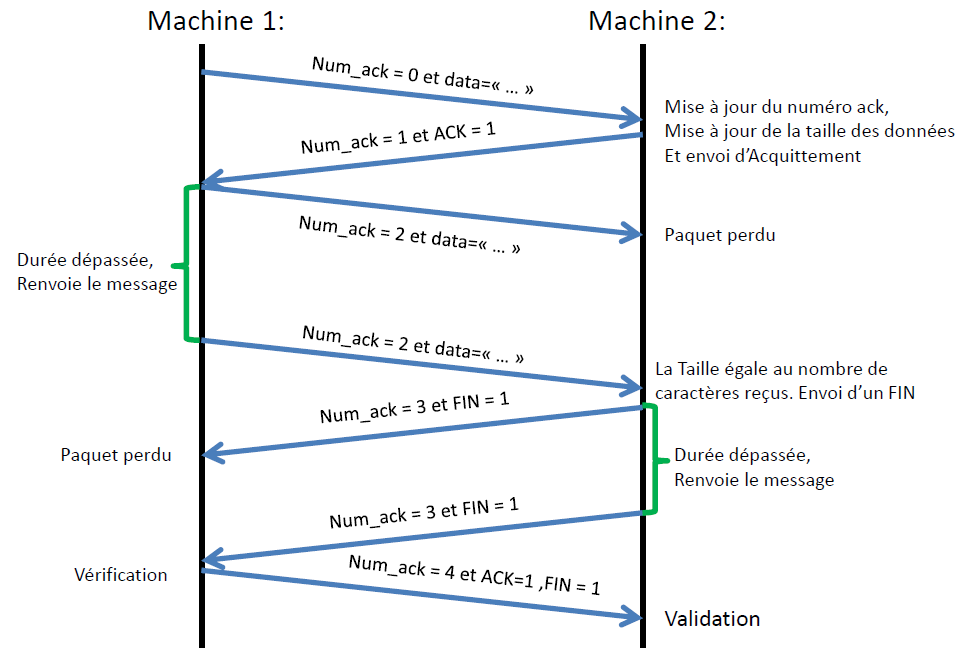
\includegraphics[scale=0.6]{protocoleReseau}
\end{center}

\bigskip


Les longs messages dépassant la taille d’une trame sont gérés par
un séquencement et l’ajout d'une taille totale dans l’en-tête de la classe MailHeader. \color{red}SEQUENCEMENT ?\color{black}
La vérification des messages via leur numéro acquittement et par leur type ACK, FIN ou donnée.\color{red}Vérification de l'authenticité de l'émetteur ? De leur ordre d'envoi ?\color{black}

\chapter{Organisation du travail en équipe}
Répartition des tâches

%Cédric : Conception et implémentation, rédaction des tests.
%Florian : Conception et implémentation.
%Hosseim : Conception et implémentation.
%Thaqif : Implémentation, rédaction des tests.
Peio : Compte rendu et exécution des tests.
Les tâches assignées à chacun montrent l’organisation générale du groupe. Cependant, toute l’équipe se tient au courant de ce que chacun fait et peut ponctuellement travailler sur la même tâche (par exemple lors de la rédaction du premier compte rendu et de la compréhension du fonctionnement des piles de thread NachOS).


\chapter{Retour global sur le projet}

[à remplir à la fin]

\end{document}